% Shared preamble for the texdocx user guide. Section files rely on these macros.
\documentclass[11pt,a4paper]{article}
\usepackage[utf8]{inputenc}
\usepackage[T1]{fontenc}
\usepackage{amsmath,amssymb,graphicx,booktabs,tabularx,longtable,multirow,enumitem,xcolor,hyperref,listings,subcaption}
\usepackage[margin=2.5cm]{geometry}
\usepackage{fancyhdr,lastpage}
\graphicspath{{figs/}}
\definecolor{accent}{HTML}{1F5FAD}
\newcommand{\texdocx}{\textsf{texdocx}}
\newcommand{\cmd}[1]{\texttt{\textbackslash#1}}
\newcommand{\env}[1]{\texttt{#1}}
\newcommand{\R}{\mathbb{R}}
\newcommand{\E}{\mathbb{E}}
\DeclareMathOperator{\argmax}{arg\,max}
\newenvironment{tip}{\begin{quote}\textbf{\textcolor{accent}{Tip.}}}{\end{quote}}

\pagestyle{fancy}
\fancyhf{}
\fancyhead[L]{\texdocx{} User Guide}
\fancyhead[R]{\leftmark}
\fancyfoot[C]{Page \thepage\ of \pageref{LastPage}}
\title{\texdocx: From \LaTeX{} to Editable Word}
\author{The \texdocx{} Project}
\date{6 October 2026}
\begin{document}
\maketitle
\begin{abstract}
This guide was written in \LaTeX{} and converted to Word by \texdocx{} itself.
Every equation in it is a native, editable Word equation; every cross-reference,
caption number and the table of contents are Word fields.
\end{abstract}
\tableofcontents
\section{Introduction}\label{sec:intro}

\texdocx{} is a compiler that turns a \LaTeX{} document into a Word file
(\texttt{.docx}). It does not run \TeX{} and it does not print to PDF first.
Instead it rebuilds the part of \LaTeX{} that \emph{reads} your source---the
tokenizer with its category codes, macro expansion, document structure and
mathematics---and hands the result to Word, which does the layout itself when
it opens the file. Line breaking, page breaking and font metrics are Word's job,
so the output reflows like any document typed in Word.

Three properties set \texdocx{} apart from converters that only approximate the
look of a \LaTeX{} paper:
\begin{itemize}
  \item \textbf{Equations stay editable.} Every formula becomes native Office
        Math (OMML), so a co-author can click into it and change a subscript in
        Word's equation editor. Section~\ref{sec:math} covers the details.
  \item \textbf{Numbers are live.} References to sections, equations,
        figures and tables, the equation and caption numbers themselves and
        the table of contents are written as Word fields with the correct value
        already filled in, so the document looks right as soon as it opens and
        Word can update the numbers after you edit it.
  \item \textbf{Your macros work.} \texdocx{} has a real macro expander, so
        \cmd{newcommand}, \cmd{def}, conditionals and environments you define
        yourself are expanded by \TeX's own rules instead of being
        matched against patterns (Section~\ref{sec:macros}).
\end{itemize}

This guide is itself a test of those claims: it was written in \LaTeX{} and
converted by \texdocx{}. Section~\ref{sec:features} surveys the supported
document features, Section~\ref{sec:figures} covers figures and tables, and
Section~\ref{sec:security} covers safety and diagnostics, including the sandbox
that keeps a document from reading anything outside its own folder.

\subsection{Quick start}

\texdocx{} needs Node.js~23.6 or newer and the pnpm package
manager.\footnote{The compiler is written in TypeScript and runs directly
through Node's built-in type stripping, which is why there is no build step and
why older Node versions are not supported.} From the repository root, install
the dependencies once and then convert a file:
\begin{lstlisting}[language=bash]
pnpm install
pnpm texdocx paper.tex                 # writes paper.docx next to it
pnpm texdocx paper.tex -o out.docx --json --strict
\end{lstlisting}

Problems are reported the way a compiler reports them: a severity, a code such
as \texttt{W013}, the file, line and column, the offending source line and,
where possible, a hint. The command accepts the following options:
\begin{description}
  \item[\texttt{-o}, \texttt{-{}-output} \textit{file}] Where to write the
        Word file. By default the output takes the input's name with the
        extension \texttt{.docx}.
  \item[\texttt{-{}-root} \textit{dir}] The folder the document may read
        from. By default this is the folder that contains the input file;
        \cmd{input} and \cmd{includegraphics} cannot reach outside it.
  \item[\texttt{-{}-strict}] Treat every warning as an error, for example to
        make a build fail on an unknown command.
  \item[\texttt{-{}-json}] Print each diagnostic as one line of JSON instead of
        the human-readable form, for editors and scripts.
  \item[\texttt{-q}, \texttt{-{}-quiet}] Print errors only.
  \item[\texttt{-h}, \texttt{-{}-help}] Show a short usage summary.
\end{description}
The exit status is~0 on success, 1 when the document had errors and 2 when the
command line was wrong or the input file could not be read. The Word file is written even when there are
errors, so you can open it and see what went wrong.

\begin{tip}
Run \texdocx{} with \texttt{-{}-strict} in continuous integration. A warning
about an unknown command usually means some text in the Word file is not what
you meant.
\end{tip}

\subsection{How it works}

\texdocx{} is designed as a pipeline of six stages. Only the first three
resemble \TeX; the last three replace \TeX's typesetter with a typed document
model and a Word writer. As in \TeX, the first four stages run interleaved,
one token at a time: the digester asks the expander for the next token, the
expander asks the lexer, and a file is loaded only when the command that
names it runs.
\begin{enumerate}
  \item \textbf{Load.} Every file the document pulls in through
        \cmd{input}, \cmd{include} or \cmd{includegraphics} is read through
        a sandbox confined to the project folder, and every token remembers
        where it came from, so a diagnostic can name the file, line and column.
  \item \textbf{Tokenize.} The lexer turns characters into tokens, looking
        up each character's category code as it reads it, so a
        \cmd{makeatletter} or \cmd{catcode} in the document changes how the
        very next character is read.
  \item \textbf{Expand.} The expander replaces macros by their definitions and
        evaluates conditionals and groups, within budgets on steps, nesting
        depth, token count and time so that a runaway macro stops with an error.
  \item \textbf{Digest.} Command and environment handlers build a document
        model of headings, paragraphs, lists, tables, figures and math trees
        instead of \TeX's boxes and glue.
  \item \textbf{Resolve.} Once the whole document has been read, every
        \cmd{ref} is matched to its \cmd{label}, so forward references work
        in a single run where \LaTeX{} needs two. An undefined reference
        prints \texttt{??} and a warning, as in \LaTeX.
  \item \textbf{Write.} The writer turns the model into Word's XML---styles,
        numbering, fields, footnotes, images and equations---and packs it into
        a byte-for-byte reproducible \texttt{.docx} archive.
\end{enumerate}
The writer depends only on the document model and never sees \LaTeX{} source,
which keeps the quirks of each format on its own side of the model.

\section{What Gets Converted}\label{sec:features}

\texdocx{} does not take a picture of a \LaTeX{} page. It reads the source,
works out what each construct \emph{means}, and then picks the closest thing
Word has for it. Sometimes Word has an exact counterpart: a \cmd{footnote}
becomes a real Word footnote, and in an article \cmd{section} becomes a paragraph in
the \emph{Heading~1} style. Sometimes it has something close but not identical, and
for a few constructs it has nothing, so \texdocx{} keeps the text and, in most
cases, warns you.
Table~\ref{tab:features-map} lists what the compiler handles today and how
faithful each conversion is.

\begin{table}[ht]
\centering
\caption{\LaTeX{} constructs and what \texdocx{} turns them into.}\label{tab:features-map}
\begin{tabularx}{\textwidth}{@{}>{\raggedright\arraybackslash}p{3.4cm}>{\raggedright\arraybackslash}p{3.6cm}l>{\raggedright\arraybackslash}X@{}}
\toprule
\LaTeX{} construct & Word representation & Fidelity & Notes \\
\midrule
\cmd{chapter} \ldots{} \cmd{subparagraph} & Heading~1--6 styles & Native & The class's top level (\cmd{chapter} or \cmd{section}) is Heading~1. Numbers come from a Word multilevel list and match \LaTeX's; starred forms are unnumbered. \\
\cmd{textbf}, \cmd{emph}, \cmd{textsc}, \cmd{textcolor}, \cmd{large} & Run formatting & Native & Bold, italic, small caps, colour and size are set on the text itself. \\
Inline and display maths & Office Math (OMML) & Native & Editable in Word's equation editor; see Section~\ref{sec:math}. \\
Equation numbers & \texttt{SEQ} field on a tab stop & Approximate & The number sits at a right tab; \cmd{eqref} is a \texttt{REF} field to it. \\
\cmd{label}, \cmd{ref}, \cmd{autoref}, \cmd{cref} & Bookmark and \texttt{REF} field & Native & The cached number is already correct when the file opens. References to list items are plain internal links instead. \\
\cmd{pageref} & \texttt{PAGEREF} field & Approximate & Shows ``?'' until Word updates fields; only Word knows the page. \\
\env{itemize}, \env{enumerate} & Word bulleted and numbered lists & Native & \env{enumitem} labels, \texttt{start} and \texttt{resume} are honoured. \\
\env{description} & Hanging-indent paragraphs & Approximate & The term is bold, followed by its text. \\
\cmd{footnote} & Word footnote & Native & Links and images inside footnotes work too. \\
\cmd{href}, \cmd{url} & Hyperlink & Native & Internal targets (\cmd{hyperlink}) become bookmark links. \\
\env{tabular}, \env{tabularx}, \env{longtable} & Word table & Native & \cmd{multicolumn} and \cmd{multirow} merge cells; \env{longtable} heads repeat on each page. \\
\env{booktabs} rules & Cell borders & Approximate & Thick and thin borders; the extra vertical padding is not reproduced. \\
\env{figure}, \env{table}, \cmd{caption} & Block kept with its caption & Approximate & Captions use \texttt{SEQ} fields, but floats stay where they are written. \\
\cmd{includegraphics} (PNG, JPEG, GIF, BMP) & Inline picture & Native & Sized like \env{graphicx}; \texttt{angle} and \texttt{trim} are ignored with a warning. \\
SVG images & SVG picture & Approximate & Shown by Word~2016 and later; older readers see a blank fallback. \\
PDF and EPS images & PNG, JPEG or SVG twin, else placeholder & Lossy & See Section~\ref{sec:figures}. \\
\env{lstlisting}, \env{minted}, \env{verbatim} & Source Code paragraph & Native & Syntax colours for 28 languages; text is kept exactly. \\
\cmd{tableofcontents} & \texttt{TOC} field & Native & Filled in when Word updates fields. \\
\env{fancyhdr} headers and footers & Header and footer parts & Native & \cmd{thepage}, \cmd{leftmark} and \texttt{LastPage} become fields. \\
\env{minipage}, \cmd{parbox} & Ordinary paragraphs & Lossy & The content is kept but the box is flattened. \\
\cmd{cite} and friends & Plain text & Lossy & Shows the keys in brackets. \\
Unknown commands & Their arguments as text & Lossy & Reported as warning W013 with the source line. \\
\bottomrule
\end{tabularx}
\end{table}

The fidelity column uses three levels. They describe what a reader of the Word
file gets, not how hard the conversion was:
\begin{description}
  \item[Native] Word has a feature that does the same job, and \texdocx{} uses
    it. A co-author editing the file in Word sees ordinary Word objects:
    headings appear in the navigation pane, footnotes renumber themselves, and
    equations open in the equation editor.
  \item[Approximate] The meaning survives but the appearance or behaviour
    differs in a visible way. A figure stays next to the paragraph it was
    written after instead of floating to the top of a page; a booktabs rule is a
    border rather than a rule with its own spacing.
  \item[Lossy] Some information is dropped. The text is kept so nothing
    disappears outright, and, except for citations, the compiler prints a
    warning that points at the line in your source.
\end{description}

\subsection{Not supported yet}

A few common constructs have no handler yet. Citations are not formatted:
\cmd{cite}, \cmd{citep}, \cmd{citet} and their \env{biblatex} relatives print
the bare keys, so \texttt{\textbackslash cite\{knuth84\}} appears as
``[knuth84]'' and any page or note arguments are dropped. Bibliography
processing is planned but not started. Theorems are not supported either:
\cmd{newtheorem} is an unknown command, so a \env{theorem} environment keeps its
text but loses its ``Theorem~1'' heading and number. \env{tikzpicture} is
treated the same way, and the drawing commands inside it end up as stray text.
Finally, a \texttt{.docx} file cannot show PDF or EPS graphics as pictures, and
\texdocx{} never runs an external converter. A figure included as
\texttt{plot.pdf} therefore needs a \texttt{plot.png}, \texttt{plot.jpg} or
\texttt{plot.svg} next to it. Without one you get a placeholder.

\begin{tip}
Unknown commands and environments, flattened boxes and missing figure twins
all produce warnings. Run \texdocx{} with \texttt{-{}-strict} to turn every
warning into an error. The command then exits with a failure status, so a build
stops instead of quietly approximating.
\end{tip}

\section{Mathematics}\label{sec:math}

A common way to move \LaTeX{} mathematics into Word is to paste each equation in as a
picture or to flatten it to plain text. \texdocx{} does neither. Its math parser reads
the same expanded token stream as the rest of the document, so your own macros work inside
formulas, and it recovers the \emph{structure} of each formula (fractions, scripts, radicals,
delimiters, matrices) rather than its layout. The \texttt{docx} writer then turns that
structure into Office Math Markup Language (OMML), the format Word's own equation editor
uses. Every formula in this section is therefore a native Word equation: click on it and
you can edit it, change its font size, or copy it into another document.

\subsection{Inline and displayed formulas}

Inline math such as $e^{i\pi} + 1 = 0$ or $\R^n$ stays in the line of text, just as it does in
\LaTeX. Fractions like $\frac{a}{b}$, roots like $\sqrt{2}$ and Greek letters such as
$\alpha$, $\beta$ and $\Gamma$ all map to their OMML counterparts. A displayed equation
gets its own paragraph. The Gaussian integral is a good first example:
\begin{equation}\label{eq:math-gauss}
  \int_{-\infty}^{\infty} e^{-x^2} \, dx = \sqrt{\pi}.
\end{equation}
Because the integral has its limits attached as scripts, Word places them beside the sign,
which is also what \LaTeX{} does for \cmd{int}. Sums and products put their limits above
and below in display style:
\[
  \sum_{k=1}^{n} k = \frac{n(n+1)}{2},
  \qquad
  \lim_{n \to \infty} \left(1 + \frac{1}{n}\right)^{n} = e.
\]
Here \cmd{left} and \cmd{right} become a single OMML delimiter object, so Word grows the
parentheses with their contents. The limit under \cmd{lim} is a real lower-limit object, not a
subscript.

\subsection{Numbering and cross-references}

Equation~\eqref{eq:math-gauss} above was numbered automatically. In the Word file the number
is not plain text: it is a \texttt{SEQ Equation} field, wrapped in a bookmark named after the
\cmd{label}. The equation itself sits at a centre tab stop and the number at a right tab stop
on the same line. Each \cmd{eqref} becomes a \texttt{REF} field that points at that bookmark,
with the parentheses added around it, exactly like the reference you just read. Both fields
carry the number \texdocx{} computed as their cached value, so the document is correct as soon
as it opens; the fields are designed so that updating them in Word (F9) gives the same numbers.

Multi-line environments number each row separately. In an \env{align} environment every row
becomes its own Word paragraph, so that it can carry its own number, and \cmd{notag} (or
\cmd{nonumber}) suppresses the number of a single row:
\begin{align}
  f(x) &= (x + 1)^2 \label{eq:math-square} \\
       &= x^2 + 2x + 1 \notag \\
  f'(x) &= 2x + 2. \label{eq:math-derivative}
\end{align}
The middle row has no number, so the derivative in~\eqref{eq:math-derivative} directly follows
\eqref{eq:math-square}, just as it would in a PDF. One visible difference remains: because the rows are separate paragraphs,
Word does not yet line up the equals signs across them. In the starred forms, which
need no numbers, the rows stay in one OMML equation array and the \& marks do align.
The starred forms number nothing; here is
\env{gather*}, which centres each row on its own:
\begin{gather*}
  \binom{n}{k} = \frac{n!}{k!\,(n-k)!}, \\
  \sqrt[3]{27} = 3, \qquad \sqrt{x^2 + y^2} \geq 0.
\end{gather*}
Note that \cmd{binom} becomes a bar-less fraction inside parentheses, and the optional argument
of \cmd{sqrt} becomes the degree of an OMML radical.

\subsection{Matrices and cases}

The \env{pmatrix} and \env{bmatrix} environments become OMML matrices wrapped in round or
square delimiters:
\[
  A = \begin{pmatrix} 1 & 2 \\ 3 & 4 \end{pmatrix},
  \qquad
  I_3 = \begin{bmatrix} 1 & 0 & 0 \\ 0 & 1 & 0 \\ 0 & 0 & 1 \end{bmatrix}.
\]
A \env{cases} environment becomes a left-aligned two-column matrix behind a single opening
brace, with no closing delimiter:
\begin{equation}\label{eq:math-abs}
  |x| = \begin{cases}
    x  & \text{if}\ x \geq 0, \\
    -x & \text{otherwise.}
  \end{cases}
\end{equation}
Text inside \cmd{text} is written as normal (non-math) text in the equation, so it keeps
upright letters and its spaces, including those at the start or end of the argument, so
\verb|\text{ if }| reads exactly as it does in the PDF.

\subsection{Fonts, braces and operators}

Math alphabets are mapped to Unicode mathematical letters, which Word shows directly in the
equation:
\cmd{mathbb} gives $\mathbb{N} \subset \mathbb{Z} \subset \mathbb{Q} \subset \R$, and
\cmd{mathcal} gives $\mathcal{F}$, $\mathcal{L}$ and $\mathcal{O}(n \log n)$. The preamble of
this guide defines \cmd{R} and \cmd{E} as shorthands for $\R$ and $\E$, and they behave like
any other macro.

An \cmd{overbrace} with a superscript becomes an OMML group character with an upper limit, so
the label sits above the brace:
\begin{equation}\label{eq:math-brace}
  \overbrace{1 + 1 + \cdots + 1}^{n\ \text{terms}} = n.
\end{equation}
Operators declared with \cmd{DeclareMathOperator} are set upright as a single function name.
This guide's preamble declares \cmd{argmax}, which reads naturally in an expected-value
problem:
\begin{equation}\label{eq:math-argmax}
  \theta^{\ast} = \argmax_{\theta \in \Theta} \E\left[ \log p(x \mid \theta) \right].
\end{equation}
Because the preamble uses the unstarred form, the subscript stays to the side even in display
style, exactly as \LaTeX{} sets it; the starred \cmd{DeclareMathOperator*} would place it
underneath, like \cmd{lim}. Inline, as in $\argmax_{\theta} f(\theta)$, the subscript is
always at the side.

\begin{tip}
The numbers of equations~\eqref{eq:math-gauss} to~\eqref{eq:math-argmax}, and every reference
to them, are fields. If you rearrange equations in Word, select the whole document and press F9
to update the fields: the equation numbers are recounted and each reference follows its
bookmark.
\end{tip}

\section{Macros and Customisation}\label{sec:macros}

Many converters treat a \LaTeX{} document as a tree of known commands and give up on
anything else. \texdocx{} instead rebuilds \TeX's front end: a tokenizer with category
codes and a macro expander with grouping, conditionals, registers and counters. Your own
definitions are therefore \emph{executed}, the way \LaTeX{} would execute them, and
the Word file receives their result rather than the raw macro name. Every example
macro below is defined in this section's own source file and then used live; the code
blocks show the definitions verbatim.

\subsection{Commands with optional arguments}

\cmd{newcommand} accepts an optional first argument with a default value, just like in
\LaTeX. The following macro typesets a keyword in bold and colours it, using the accent
colour from the preamble unless another colour is given:

\begin{verbatim}
\newcommand{\keyword}[2][accent]{\textcolor{#1}{\textbf{#2}}}
\end{verbatim}
\newcommand{\keyword}[2][accent]{\textcolor{#1}{\textbf{#2}}}

Writing \verb|\keyword{expansion}| gives \keyword{expansion}, while
\verb|\keyword[accent!50]{tint}| gives \keyword[accent!50]{tint}. The second form uses an
\texttt{xcolor} mixing expression: \texttt{accent!50} is half accent and half white, and
\texttt{accent!60!black} would mix the accent with black instead. \texdocx{} evaluates
these expressions itself and writes the resulting RGB value into the run, so
\textcolor{accent}{plain accent text} and \textcolor{accent!50}{the lighter mix} both
survive as ordinary Word font colours that you can change later.

\subsection{Environments}

\cmd{newenvironment} works with arguments and an optional default, and the end code runs
before the environment name is checked, as in \LaTeX:

\begin{verbatim}
\newenvironment{aside}[1][Aside]
  {\par\medskip\noindent\textcolor{accent}{\textbf{#1.}}\ \itshape}
  {\par\medskip}
\end{verbatim}
\newenvironment{aside}[1][Aside]
  {\par\medskip\noindent\textcolor{accent}{\textbf{#1.}}\ \itshape}
  {\par\medskip}

\begin{aside}[Why it matters]
Declarations such as \cmd{itshape} inside an environment are local to it. This
paragraph is italic; the one after the environment is not.
\end{aside}

Back to upright text: the group opened by \verb|\begin{aside}| was closed by
\verb|\end{aside}|, and the font change went with it.

\subsection{Star arguments with xparse}

\cmd{NewDocumentCommand} takes an argument specification instead of a count. Below,
\texttt{s} is an optional star, \texttt{m} a mandatory argument and \texttt{o} an
optional bracketed argument with no default:

\begin{verbatim}
\NewDocumentCommand{\concept}{s m o}{%
  \IfBooleanTF{#1}{\emph{#2}}{\textbf{#2}}%
  \IfValueT{#3}{ (#3)}}
\end{verbatim}
\NewDocumentCommand{\concept}{s m o}{%
  \IfBooleanTF{#1}{\emph{#2}}{\textbf{#2}}%
  \IfValueT{#3}{ (#3)}}

So \verb|\concept{catcode}| prints \concept{catcode}, \verb|\concept*{catcode}| prints
\concept*{catcode}, and \verb|\concept{OMML}[Office Math]| prints
\concept{OMML}[Office Math]. \cmd{NewDocumentEnvironment}, including the \texttt{b}
argument that captures the whole body, is supported as well.

\subsection{Primitive definitions}

Plain \TeX{} definitions work too. A \cmd{def} may use \emph{delimited} parameters, where the
text between parameters must appear literally in the input:

\begin{verbatim}
\def\interval[#1..#2]{$[#1,#2]$}
\end{verbatim}
\def\interval[#1..#2]{$[#1,#2]$}

Here \verb|\interval[0..1]| becomes \interval[0..1] and \verb|\interval[a..b]| becomes
\interval[a..b]: the expander matched the two dots and the closing bracket to split the
arguments. Switches made with \cmd{newif} behave like their \TeX{} counterparts:

\begin{verbatim}
\newif\ifshowhints
\showhintstrue  \ifshowhints Hints are on.\else Hints are off.\fi
\showhintsfalse \ifshowhints Hints are on.\else Hints are off.\fi
\end{verbatim}
\newif\ifshowhints

After \verb|\showhintstrue| the test prints
``\showhintstrue\ifshowhints Hints are on.\else Hints are off.\fi'' and after
\verb|\showhintsfalse| it prints
``\showhintsfalse\ifshowhints Hints are on.\else Hints are off.\fi'' instead. Other primitives
such as \cmd{edef}, \cmd{let}, \cmd{expandafter}, \cmd{csname} and \cmd{ifx} are
available for the same kind of programming.

\begin{tip}
All expansion runs under budgets for expansion steps, nesting depth, token count and
wall-clock time. A runaway recursive macro therefore stops with error E003, which names
the macro stack, instead of hanging the conversion. A command that is not defined at all
is reported as warning W013, and its arguments are kept as text.
\end{tip}

\subsection{Counters and cross-references}

Custom counters take part in the same numbering machinery as sections and equations. The
counter below resets with every section, and its printed form is redefined to show
the section number followed by a capital letter:

\begin{verbatim}
\newcounter{checkpoint}[section]
\renewcommand{\thecheckpoint}{\thesection.\Alph{checkpoint}}
\newcommand{\checkpoint}[1]{\par\noindent
  \refstepcounter{checkpoint}\textbf{Checkpoint \thecheckpoint.} #1\par}
\end{verbatim}
\newcounter{checkpoint}[section]
\renewcommand{\thecheckpoint}{\thesection.\Alph{checkpoint}}
\newcommand{\checkpoint}[1]{\par\noindent
  \refstepcounter{checkpoint}\textbf{Checkpoint \thecheckpoint.} #1\par}

\checkpoint{The document compiles without errors.}\label{cp:macros-compiles}
\checkpoint{Every label is referenced at least once.}\label{cp:macros-labels}

Because \cmd{refstepcounter} sets the current label, \verb|\ref{cp:macros-labels}|
yields \ref{cp:macros-labels} and \verb|\ref{cp:macros-compiles}| yields
\ref{cp:macros-compiles}, the same text that \LaTeX{} prints. Note that the format,
including the section prefix, comes from your redefinition of \cmd{thecheckpoint}.

\subsection{Customised lists}

The \texttt{enumitem} keys are read too. A list can choose its own label format and a
later list can continue where it stopped, with \texttt{resume*} also reusing the first
list's options:

\begin{verbatim}
\begin{enumerate}[label=(\alph*)]
  \item Write the macro.
  \item Use it in the text.
\end{enumerate}
\begin{enumerate}[resume*]
  \item Check the output.
\end{enumerate}
\end{verbatim}

The live version, with a paragraph between the two lists:

\begin{enumerate}[label=(\alph*)]
  \item Write the macro in the preamble or before its first use.\label{it:macros-write}
  \item Use it in the text as often as needed.
\end{enumerate}
Then compile the document and open the result in Word.
\begin{enumerate}[resume*]
  \item Check the output: the numbering continues with the same format.\label{it:macros-check}
\end{enumerate}

Item references follow the label format, so \verb|\ref{it:macros-check}| gives
\ref{it:macros-check} and \verb|\ref{it:macros-write}| gives \ref{it:macros-write}.

\subsection{Limits}

Code inside \cmd{ExplSyntaxOn}\,\dots\,\cmd{ExplSyntaxOff} is not interpreted; the block
is skipped with warning W015. A package that \texdocx{} does not know is reported as
W010. Packages that are accepted without a warning do not
necessarily implement every one of their commands, and an unknown command still produces
W013. The commands that \texdocx{} recognises are listed in
\texttt{docs/supported-commands.md}. Section~\ref{sec:features} gives an overview of the
other document features, and Section~\ref{sec:security} explains the sandbox in which all
of this expansion runs.

\section{Figures and Tables}\label{sec:figures}

Figures and tables are where \LaTeX{} and Word differ most. \LaTeX{} moves a float to
the top of a page, the bottom of a page or a page of its own; Word has nothing comparable. \texdocx{} therefore writes every \env{figure} and \env{table} where it
appears in the source, accepts and ignores the placement specifier (\texttt{[htbp]} and
friends), and marks every paragraph of the float before its last caption as
\emph{keep with next}, so an image never ends up on one page with its caption on the
next. What you get is a document a co-author can edit without fighting anchored frames.

\subsection{Images and how they are sized}\label{sec:figures-sizing}

\cmd{includegraphics} follows the \textsf{graphicx} rules, so an image is as large in Word
as it would be in the PDF. The starting point is the image's natural size, computed from
its pixel dimensions and the resolution stored in the file: the \texttt{pHYs} chunk of a
PNG or the density in a JPEG's JFIF header, and 72\,dpi when the file records none,
which is what pdf\TeX{} assumes too. An SVG's natural size comes from its \texttt{width}
and \texttt{height} attributes or, failing those, its \texttt{viewBox}. The options then
apply in the usual way:
\begin{itemize}
  \item \texttt{scale} multiplies the natural size;
  \item \texttt{width} or \texttt{height} alone sets that dimension and scales the other
        to preserve the aspect ratio (\texttt{totalheight} is treated like \texttt{height});
  \item \texttt{width} and \texttt{height} together stretch the image to exactly that box,
        unless \texttt{keepaspectratio} is given, in which case it is scaled to the
        largest size that fits inside the box.
\end{itemize}
Lengths may use any unit and any length register: \cmd{textwidth} and \cmd{linewidth} are
derived from the page set up with \textsf{geometry}, and inside a \env{subfigure} or
\env{minipage} \cmd{linewidth} is the width of that box. After sizing, one rule is
specific to \texdocx: an image wider than the text block is scaled down, keeping its
aspect ratio, to the text width. \LaTeX{} would let it run into the margin with an
\emph{overfull box} warning; Word would let it run off the page. Give the size to
\cmd{includegraphics} itself: \cmd{scalebox} and \cmd{resizebox} around an image are
currently ignored, so the image keeps its own size, and no warning is printed.

Figure~\ref{fig:figures-bars} was included with \verb|width=0.7\linewidth|. Its file is
600 pixels wide and records 150\,dpi, so its natural width is 4\,inches (about
10.2\,cm); the explicit width scales it to 70\,\% of the 16\,cm line, 11.2\,cm, exactly
as in the PDF.

\begin{figure}[htbp]
  \centering
  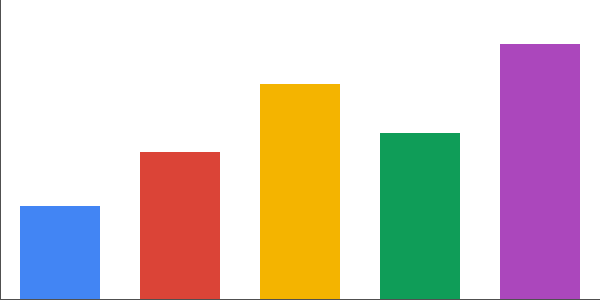
\includegraphics[width=0.7\linewidth]{bars}
  \caption{A bar chart included at 70\,\% of the line width.}\label{fig:figures-bars}
\end{figure}

Images are looked up in the project folder (by default the folder of the main file) and
in every directory named by
\cmd{graphicspath}; a name without an extension is tried as \texttt{.png}, \texttt{.jpg},
\texttt{.jpeg}, \texttt{.gif}, \texttt{.svg}, \texttt{.bmp}, \texttt{.pdf} and
\texttt{.eps}, in that order. Like every other file a document reads, images must lie
inside the project folder (Section~\ref{sec:security}). PNG, JPEG, GIF, BMP and SVG are
embedded as they are; SVG images carry a blank PNG fallback, because \texdocx{} bundles no
rasteriser, so they display in Word 2016 and later. Word cannot embed PDF or EPS
graphics, so for those \texdocx{} looks for a PNG, SVG or JPEG \emph{twin} with the same
base name and uses it instead; it never runs an external converter.
Table~\ref{tab:figures-formats} summarises the rules. Rotation (\texttt{angle}) and
cropping (\texttt{trim}, \texttt{viewport}) are not applied yet and produce warning
\texttt{W014}.

\begin{table}[htbp]
  \centering
  \caption{How each image format is sized and embedded.}\label{tab:figures-formats}
  \begin{tabular}{@{}lll@{}}
    \toprule
    & \multicolumn{2}{c}{Handling} \\
    \cmidrule(l){2-3}
    Format & Natural size from & Embedded as \\
    \midrule
    PNG & pixels and \texttt{pHYs} resolution & the PNG itself \\
    JPEG & pixels and JFIF density & the JPEG itself \\
    GIF, BMP & pixels at 96\,dpi (BMP: stored resolution) & the file itself \\
    SVG & \texttt{width}/\texttt{height} or \texttt{viewBox} & SVG with blank PNG fallback \\
    \multirow{2}{*}{PDF, EPS} & twin found: the twin's size & the twin \\
    & no twin & placeholder and \texttt{W014} \\
    \bottomrule
  \end{tabular}
\end{table}

\subsection{Subfigures}\label{sec:figures-subfigures}

The \textsf{subcaption} package's \env{subfigure} environment works as in \LaTeX: each
panel gets its own caption, lettered (a), (b), \dots, and a \cmd{label} placed after a
subcaption refers to the panel. Figure~\ref{fig:figures-pair} contains two panels: the
vector diagram in Figure~\ref{fig:figures-diagram} and the photograph in
Figure~\ref{fig:figures-photo}. As in \LaTeX, a reference to a panel combines the figure
number with the panel letter. Two differences remain. Panels are stacked vertically
rather than placed side by side, so leave out the \cmd{hfill} that usually separates
them; \texdocx{} would only approximate it with a tab and warn. And a reference to a panel
is written as plain text such as ``2a'' rather than as a field, so it is not renumbered
when fields are updated in Word.

\begin{figure}[htbp]
  \centering
  \begin{subfigure}{0.45\linewidth}
    \centering
    
\includegraphics[width=\linewidth]{diagram.svg}
    \caption{A vector diagram (SVG).}\label{fig:figures-diagram}
  \end{subfigure}
  \begin{subfigure}{0.45\linewidth}
    \centering
    
\includegraphics[width=0.8\linewidth]{photo}
    \caption{A photograph (JPEG).}\label{fig:figures-photo}
  \end{subfigure}
  \caption{Two panels in one figure.}\label{fig:figures-pair}
\end{figure}

\subsection{Captions, references and lists}\label{sec:figures-captions}

A caption's number is not typed into the document as plain text. ``Figure~1'' is the word
\emph{Figure}, a non-breaking space and the Word field \verb|SEQ Figure \* ARABIC|, with
the number \LaTeX{} would print stored as the field's cached result; tables use
\verb|SEQ Table|. A \cmd{label} after the caption becomes a bookmark around that field, and
\cmd{ref} becomes a \texttt{REF} field pointing to it, so if a figure is added or deleted
in Word, updating fields (select all, then \textsf{F9}) renumbers the captions and every
reference to them, except the panel references described above. A table caption may come above the table, as in
Table~\ref{tab:figures-formats}; it is then kept with the table that follows it.

For the same reason, \cmd{listoffigures} and \cmd{listoftables} do not produce a static
list. Each inserts a heading and a Word table-of-contents field built from the caption
fields, \verb|TOC \h \z \c "Figure"| or \verb|TOC \h \z \c "Table"|, which Word fills in
the next time fields are updated. This guide does not include one, but a document that
does gets clickable entries with page numbers computed by Word's own layout.

\begin{tip}
Give every float a \cmd{label} placed \emph{after} its \cmd{caption}. A label placed
before the caption picks up the number of the current section or subsection
instead, in \LaTeX{} and in \texdocx{} alike.
\end{tip}

\section{Safety and Diagnostics}\label{sec:security}

A \LaTeX{} file is a program, not just a document. Compiling one with a
traditional \TeX{} engine can read arbitrary files, write new ones and, with
shell escape enabled, run commands on your machine. \texdocx{} is designed to
convert documents you did not write: papers from co-authors, submissions,
templates downloaded from the web. It therefore treats every input as
untrusted. It does not call a \TeX{} engine at all; it reimplements the
\LaTeX{} front end (tokenizer, macro expansion, document structure) and only
ever produces a \texttt{.docx} file.

\subsection{Sandbox guarantees}\label{sec:security-sandbox}

The following properties hold for every document, whatever macros it defines.
The project's security test suite checks the main ones on every test run.

\begin{itemize}
  \item \textbf{Root confinement.} \cmd{input}, \cmd{include}, \cmd{subfile}
    and \cmd{includegraphics} can read only files inside the project folder:
    by default the folder of the main file, or the folder given with
    \verb|--root|. Absolute paths, paths starting with \verb|~| and \verb|../|
    escapes are refused with error E004. Such paths are rejected on their text
    alone, before any file is looked up, so the file system outside the
    project is not touched. The
    refusal reads the same whether the outside file exists or not, so a
    document cannot use it to discover your files.
  \item \textbf{Symbolic links.} Every candidate file is resolved to its real
    path before it is opened. A link inside the project that points outside
    it is refused exactly like a \verb|../| path.
  \item \textbf{Restricted file types.} Source commands read
    \texttt{.tex}, \texttt{.ltx}, \texttt{.bbl}, \texttt{.tikz} and
    \texttt{.pgf} files; \cmd{includegraphics} reads only image formats
    (PNG, JPEG, GIF, BMP, SVG, PDF, EPS, PS). A file with any other extension,
    such as \texttt{.key} or \texttt{.json}, is refused with E004 even when
    it lies inside the project. A file with \emph{no} extension is still
    read, as in \LaTeX{}, where \verb|\input{chapter}| falls back to a file
    named \texttt{chapter}; at present this also lets dotfiles such as
    \texttt{.env} through.
  \item \textbf{No shell.} \cmd{write18} is recognised and ignored with
    warning W017; no command is ever executed. For the same reason, PDF and
    EPS figures are not converted with external tools: \texdocx{} uses a PNG,
    SVG or JPEG file of the same name if one exists, and otherwise inserts a
    placeholder.
  \item \textbf{No file writes.} \cmd{openout} is ignored with warning W016.
    The only file written is the \texttt{.docx} you asked for.
  \item \textbf{No network.} A file name that looks like a URL is refused as a
    remote resource. Links made with \cmd{href} and \cmd{url} are copied
    into the Word file as hyperlinks; they are never fetched.
  \item \textbf{Resource budgets.} Macro expansion is limited to 5\,000\,000
    steps, a nesting depth of 10\,000, 50\,000\,000 tokens and 60 seconds of
    wall-clock time. Each file the document reads may be at most 20\,MiB,
    and one run reads at most 2\,000 files. A macro bomb such as \verb|\def\a{\a\a}\a| stops with
    error E003, which names the macro stack that ran away; the text converted
    up to that point is kept.
\end{itemize}

Text from the document is always escaped before it reaches the Word XML, so
words such as \texttt{INCLUDETEXT} or \texttt{DDE} in the source remain plain
text and cannot turn into active Word fields.

\begin{tip}
The sandbox protects everything outside the project folder. Treat the folder
itself as readable by the document, because the type check does not stop
files without an extension: keep credentials, \texttt{.env} files and
private keys somewhere else, and point \verb|--root| at the smallest folder
that holds the sources and figures.
\end{tip}

\subsection{Why there is no shell at all}\label{sec:security-shell}

Many \TeX{} installations allow a restricted shell escape that runs only a
list of trusted programs. That design depends on every engine enforcing the
list correctly, and it has failed in practice.
\href{https://nvd.nist.gov/vuln/detail/cve-2023-32700}{CVE-2023-32700}
describes how LuaTeX before version 1.17.0 let a document reach the original
\texttt{io.popen} function and so run arbitrary shell commands while
compiling an untrusted file. The National Vulnerability Database rates it
CVSS~3.1 base score 7.8 (High). The fix is to upgrade to LuaTeX 1.17.0 or
later; for distributions, that means TeX Live 2023 from revision 66984 on,
or MiK\TeX{} 23.5 and newer. \texdocx{} avoids this whole class of
problem by having no code path that starts a process: there is no allow-list
to bypass.

\subsection{Risks and recommended actions}\label{sec:security-risks}

Table~\ref{tab:security-risks} lists the main risks of converting an
untrusted document and what to do about each. The severity column is the
\texdocx{} project's own rating of the impact if the risk were not handled;
only the CVE row carries an official CVSS score.

\begin{table}[ht]
  \centering
  \caption{Risks of converting untrusted \LaTeX{} and how they are handled.}
  \label{tab:security-risks}
  \begin{tabularx}{\textwidth}{XlX}
    \toprule
    \textbf{Risk} & \textbf{Severity} & \textbf{Recommended action} \\
    \midrule
    Shell escape (\cmd{write18}, CVE-2023-32700) & High & None in \texdocx{} (never run, W017); patch \TeX{} installs \\
    Reading files outside the project & High & Keep \verb|--root| at the project folder; E004 blocks escapes \\
    Reading secrets inside the project (dotfiles, files without extension) & Medium & Keep secrets out of the \verb|--root| folder \\
    Symbolic links leaving the project & High & None needed; real paths are checked \\
    Writing files (\cmd{openout}) & Medium & None needed; ignored with W016 \\
    Fetching remote resources & Medium & None needed; URLs are refused with E004 \\
    Macro bombs, runaway recursion & Medium & Rely on budgets (E003); add a process timeout on servers \\
    Silently lost content & Low & Review W013 and W014, or use \verb|--strict| \\
    \bottomrule
  \end{tabularx}
\end{table}

\subsection{Reading diagnostics}\label{sec:security-diagnostics}

\texdocx{} reports problems in the style of a modern compiler: a severity and
a stable code, a message, the file, line and column, the offending source
line with a caret under the exact spot, and often a hint. The following
output comes from a short file that uses an undefined macro and tries to
read a file outside its folder:

\begin{verbatim}
warning[W013]: unknown command \highlightbox, rendered its arguments as text
 --> report.tex:3:13
  |
3 | Results are \highlightbox{significant} at $p<0.05$.
  |             ^^^^^^^^^^^^^
  = hint: define it with \newcommand or add a package handler

error[E004]: \input{../secret}: the file is outside the project folder
 --> report.tex:4:1
  |
4 | \input{../secret}
  | ^
\end{verbatim}

The run still writes a \texttt{.docx}, but exits with status 1 because there
was an error. With \verb|--json| each diagnostic is printed as one JSON
object per line, which is convenient for editors and continuous integration;
\verb|--strict| turns every warning into an error. Three codes are worth
knowing:

\begin{description}
  \item[W013 (unknown command)] \texdocx{} has no handler for the command and
    no definition was found. Its brace arguments are kept as ordinary text,
    but an optional argument in square brackets is dropped, and the
    formatting the command would have applied is lost. Define the command with \cmd{newcommand} in your preamble, or check
    for a typo.
  \item[W014 (unsupported feature approximated)] The construct was understood
    but has no exact Word equivalent, so \texdocx{} approximated it. Examples
    are a PDF figure replaced by a placeholder, \cmd{hfill} turned into a tab,
    or an image rotation that is not applied. Read the message and check that
    spot in the Word file.
  \item[E004 (file access denied)] A file request broke a sandbox rule: it
    was outside the project, an absolute path, a URL, a file type the
    command may not read, or over a size or file-count limit. The file is never opened: a refused \cmd{input} inserts nothing, and a
    refused figure appears as a placeholder that names the file.
    Move the file into the project folder or change \verb|--root|.
\end{description}

\end{document}
